\chapter{Results}
In this chapter we will present models created during the project.
We will also present the choosing criteria for the best model and we will evaluate the model on the testing data.
Then we will presents the results.

\section{Pipeline}
During this project we created a reproducible pipeline.
This pipeline is able to download the required data and preprocess them in the way that is suitable as an input to the neural networks models.
The pipeline is then able to create a model based on our specification and train it on the training dataset.

\section{Model comparison}

\subsection{PCA vs. genes vs. pathways}
\subsection{Input size}
\subsection{Tissue type and stages}
The tissue type prediction problem seem to be relatively easy from the expression data.
Although we achieved really good accuracy, we noticed that the best model was simple model without any hidden layer, which can be reduced to simple linear model.

\begin{figure}
    \centering
    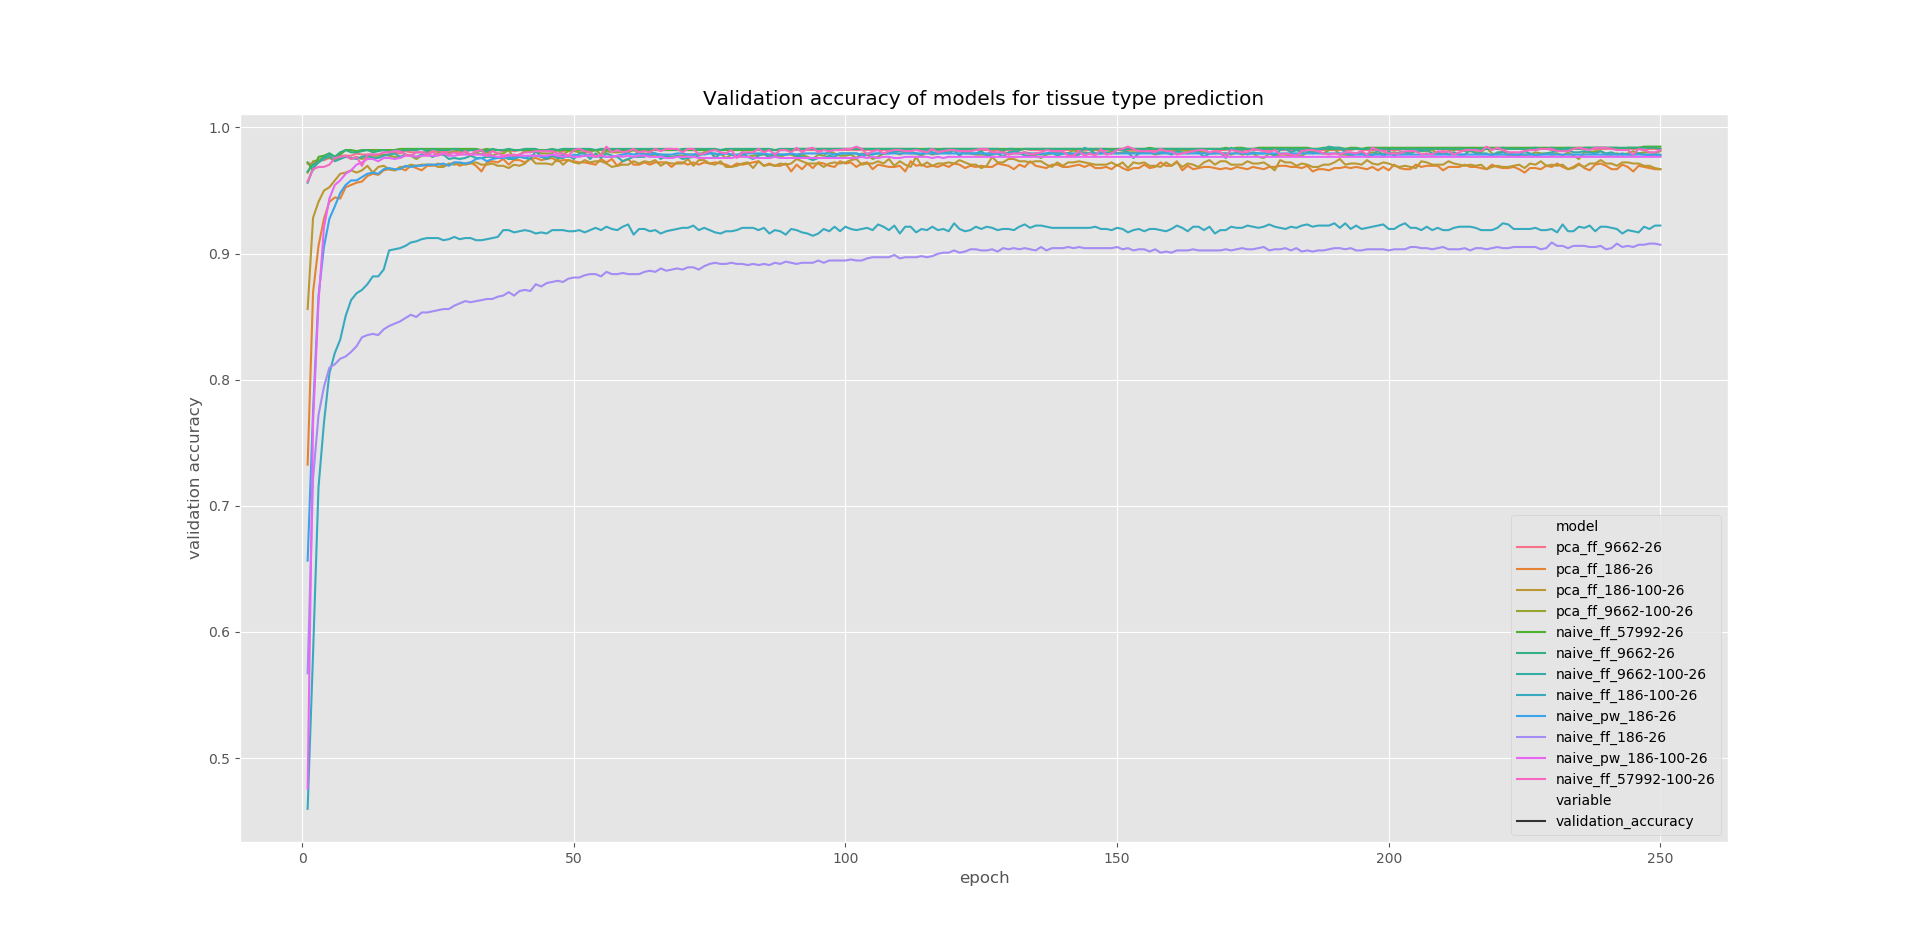
\includegraphics[width=\linewidth]{images/val_acc_tt.png}
    \caption{Caption}
    \label{fig:val_acc_tt}
\end{figure}

\begin{figure}
    \centering
    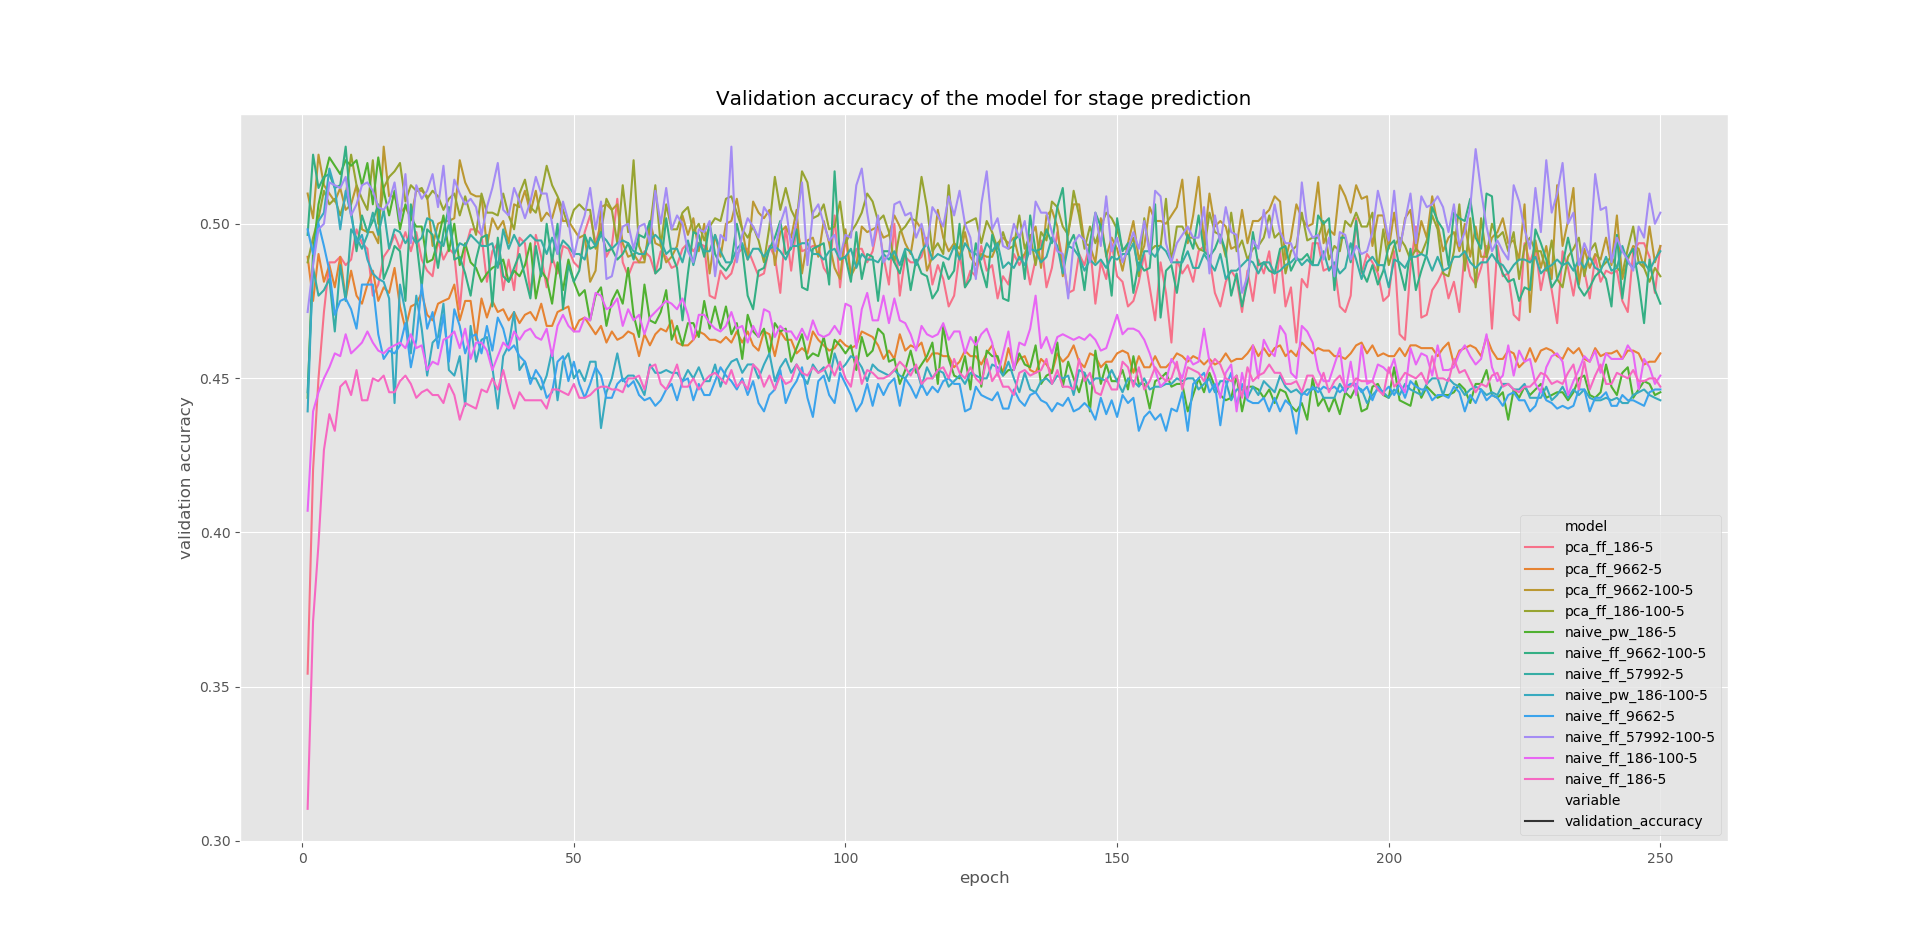
\includegraphics[width=\linewidth]{images/val_acc_st.png}
    \caption{Caption}
    \label{fig:val_acc_st}
\end{figure}

% Unfortunatelly, L2 regularization did not improve our accuracy over the model with just dropout, therefore we decided not to use it.
